\documentclass{article}
\usepackage[utf8]{inputenc}
\usepackage{fancyhdr}
\usepackage{graphicx}
\usepackage{hyperref}

\title{\textbf{Debian LTS Survey}}
\author{Utkarsh Gupta \\
    \small (utkarsh@debian.org)}
\date{August 15th 2020}

\addtolength{\oddsidemargin}{-.875in}
\addtolength{\evensidemargin}{-.875in}
\addtolength{\textwidth}{1.75in}

\addtolength{\topmargin}{-.875in}
\addtolength{\textheight}{1.75in}

\begin{document}

\maketitle

\vspace{5mm}
\section{Introduction}

On July 18th, Stretch LTS started, offering two more years of security support to the Debian Stretch
release. Stretch LTS is the fourth iteration of LTS, following Squeeze LTS which started in 2014,
Wheezy LTS in 2016, and Jessie LTS in 2018. \par

\vspace{3mm}
However, for the first time, we prepared a small survey about our users and contributors, who they
are and why they are using LTS. This document compiles the results of that very survey.

\vspace{5mm}
\section{Quick Statistics}

\vspace{3mm}
\begin{itemize}
    \item Number of questions: 14
    \item Survey duration: 2 weeks
    \item Survey start date: July 13th, 2020
    \item Survey end date: July 27th, 2020
    \item Total responses: 1764
    \begin{itemize}
        \item Complete responses: 892
        \item Incomplete responses: 872
    \end{itemize}
\end{itemize}
\textbf{NOTE}: ``Incomplete responses'' are the surveys that the user started fulfilling and then went
to another place saving for later or even not saving, i.e., data stored but without the user clicking
the ``submit'' button. ``Complete responses'' are the surveys that the user sent by clicking
the ``submit'' button (they can include some unanswered questions, if they were optional).
More info at \href{https://manual.limesurvey.org/Responses}{https://manual.limesurvey.org/Responses}.

\vspace{3mm}
\section{Responses}

\vspace{3mm}
We've got an overwhelming response from the survey. Below are the compiled responses and the stats.

\vspace{3mm}
\subsection{Objective Questions}

\vspace{3mm}
11 out of 14 questions were objective in nature. They are statistically represented with the help
of a bar graph or a pie chart and are as follows.

\newpage

\Large{\textbf{Question 1: Who are you?}}

\vspace{3mm}
\begin{figure}[h!]
\centering
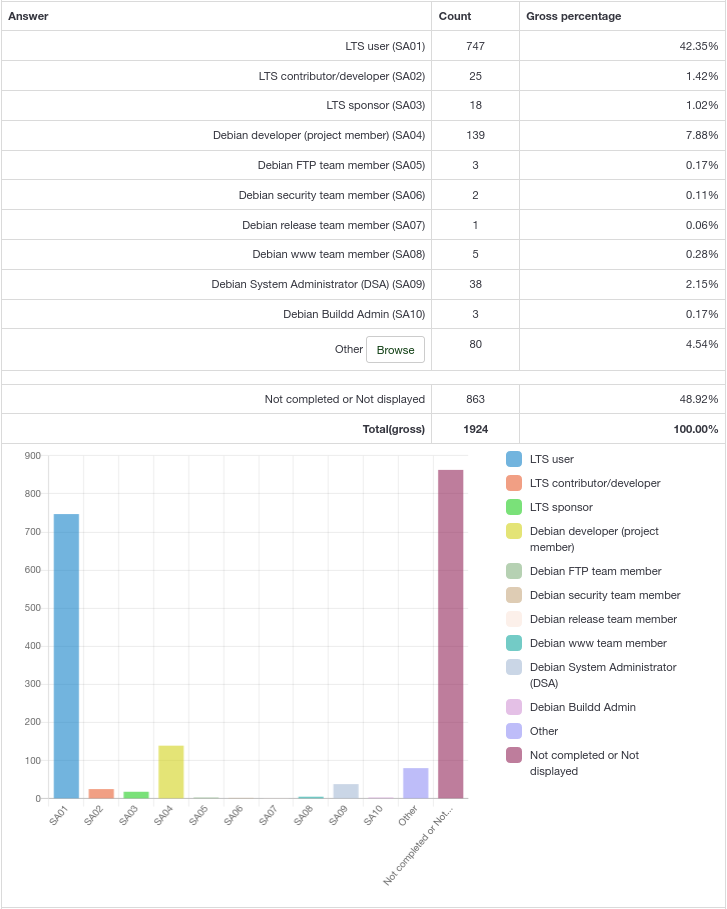
\includegraphics[width=16.9cm]{assets/1-summary.png}
\caption{Summary of Response 1}
\end{figure}

\newpage

\Large{\textbf{Question 2: How long have you been using Debian?}}

\vspace{3mm}
\begin{figure}[h!]
\centering
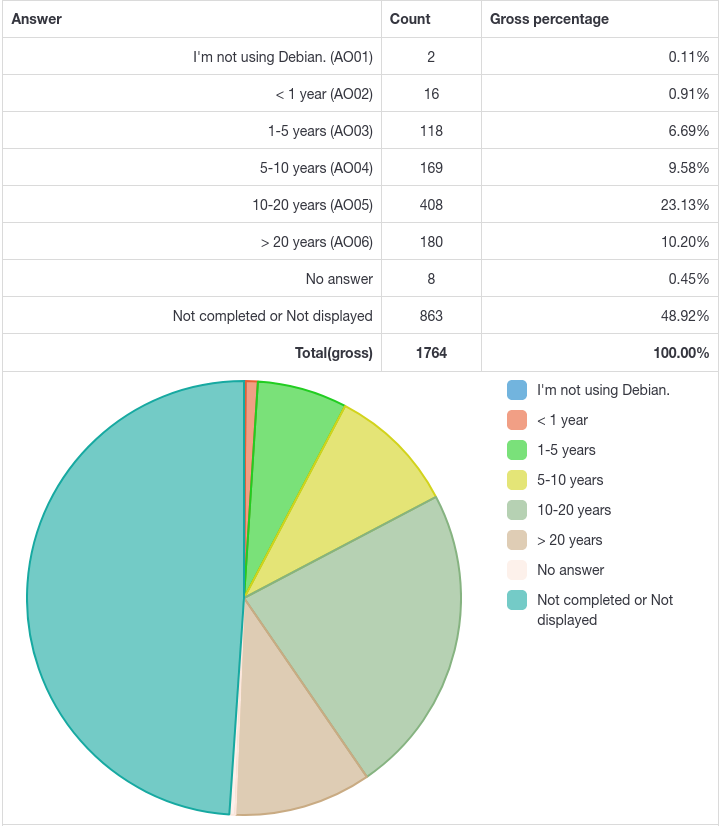
\includegraphics[width=16.5cm]{assets/2-summary.png}
\caption{Summary of Response 2}
\end{figure}

\newpage

\Large{\textbf{Question 3: How long have you been using LTS?}}

\vspace{3mm}
\begin{figure}[h!]
\centering
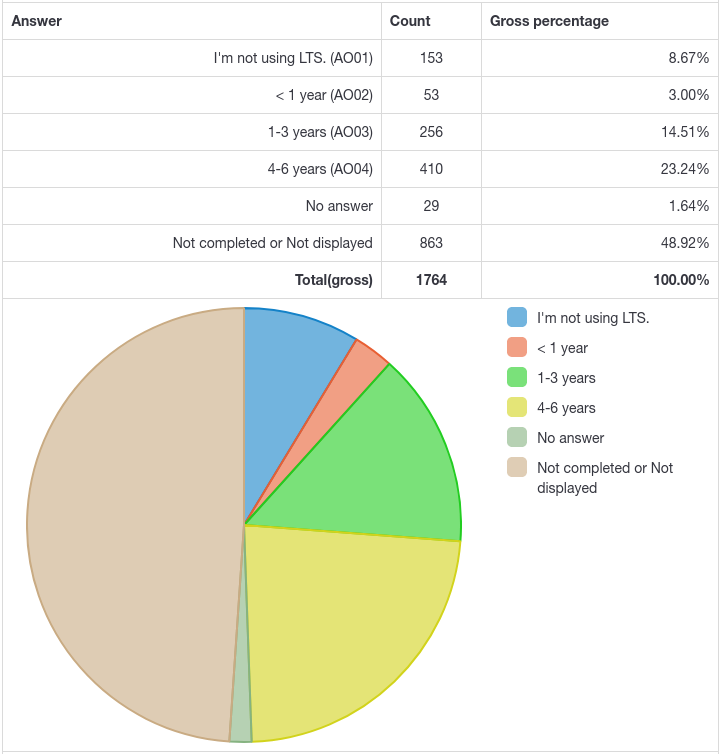
\includegraphics[width=16.5cm]{assets/3-summary.png}
\caption{Summary of Response 3}
\end{figure}

\newpage

\Large{\textbf{Question 4: Are you using Extended LTS (ELTS)?}}

\vspace{3mm}
\begin{figure}[h!]
\centering
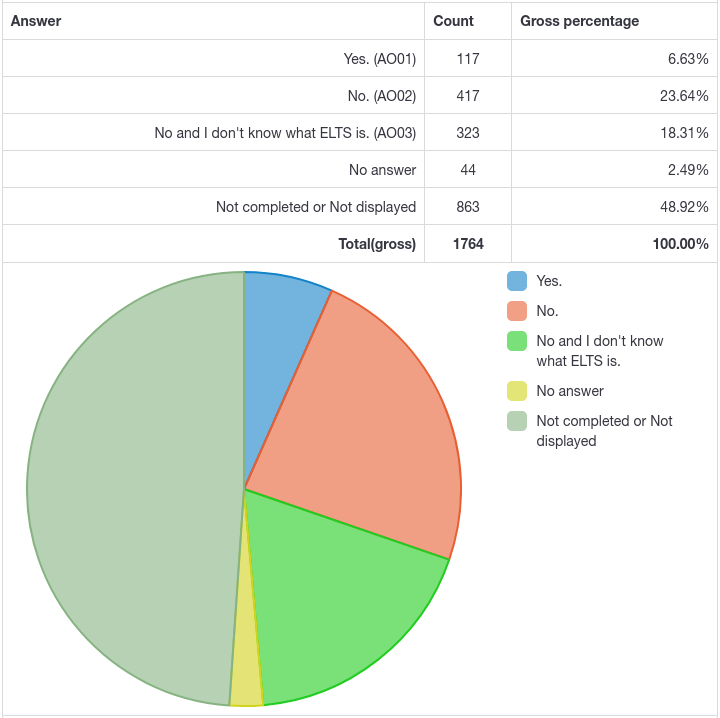
\includegraphics[width=16.5cm]{assets/4-summary.png}
\caption{Summary of Response 4}
\end{figure}

\newpage

\Large{\textbf{Question 5: On a scale of 1 (= very unhappy) to 10 (= very happy) how happy are you with
the quality of the LTS updates?}}

\vspace{3mm}
\begin{figure}[h!]
\centering
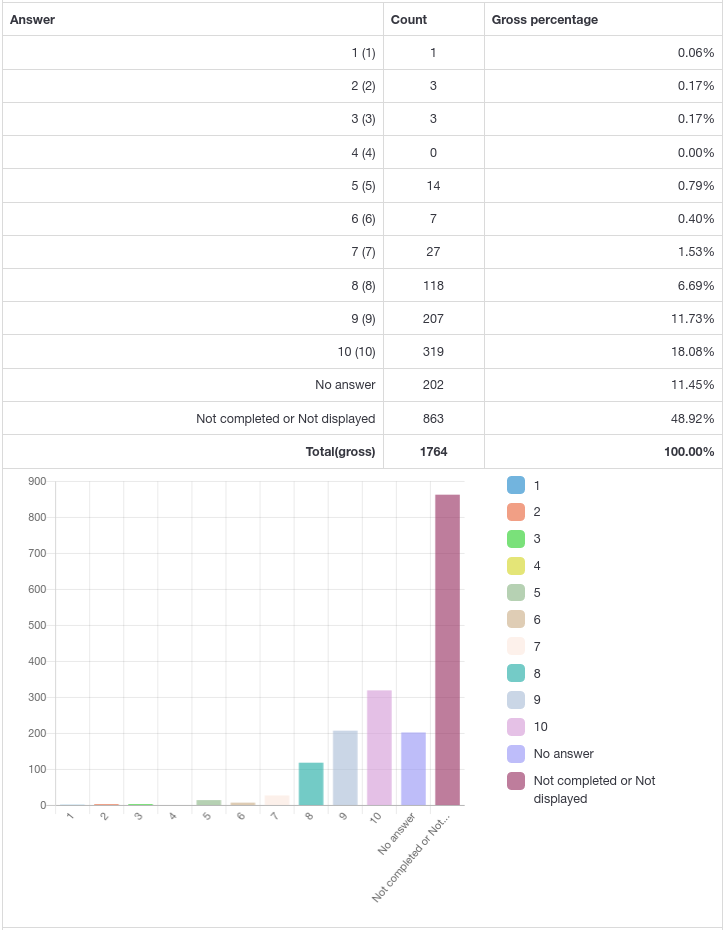
\includegraphics[width=16.3cm]{assets/5-summary.png}
\caption{Summary of Response 5}
\end{figure}

\newpage

\large{\textbf{Question 6: On a scale of 1 (= very unhappy) to 10 (= very happy), how happy are you with
how quickly LTS updates reach you?}}

\vspace{3mm}
\begin{figure}[h!]
\centering
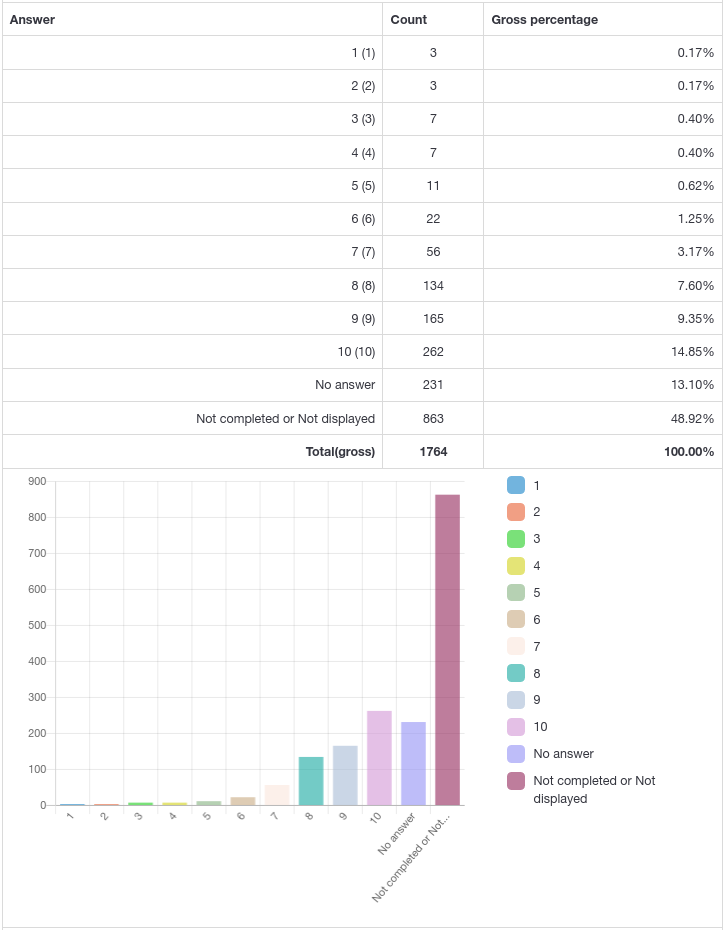
\includegraphics[width=16.5cm]{assets/6-summary.png}
\caption{Summary of Response 6}
\end{figure}

\newpage

\Large{\textbf{Question 7: How would you feel if you could no longer use Debian LTS?}}

\vspace{3mm}
\begin{figure}[h!]
\centering
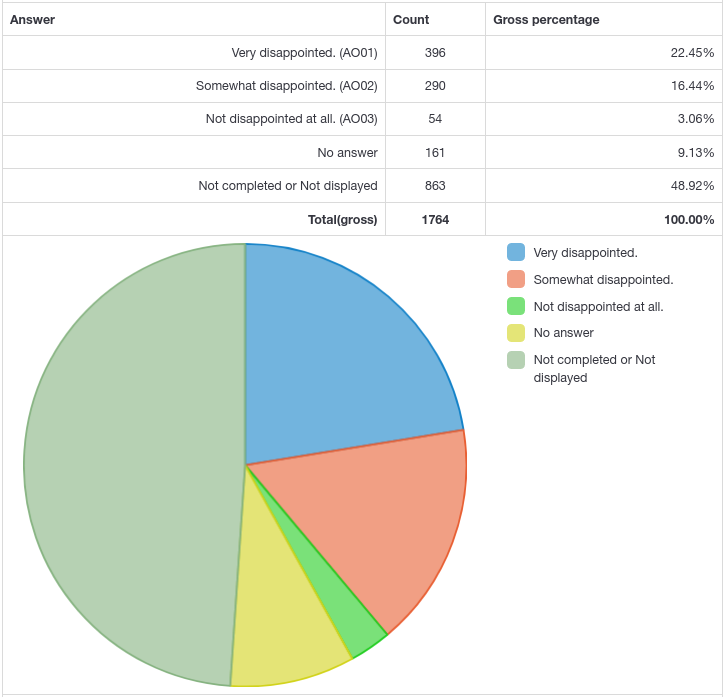
\includegraphics[width=16.5cm]{assets/7-summary.png}
\caption{Summary of Response 7}
\end{figure}

\newpage

\Large{\textbf{Question 8: Where do you use Debian LTS?}}

\vspace{3mm}
\begin{figure}[h!]
\centering
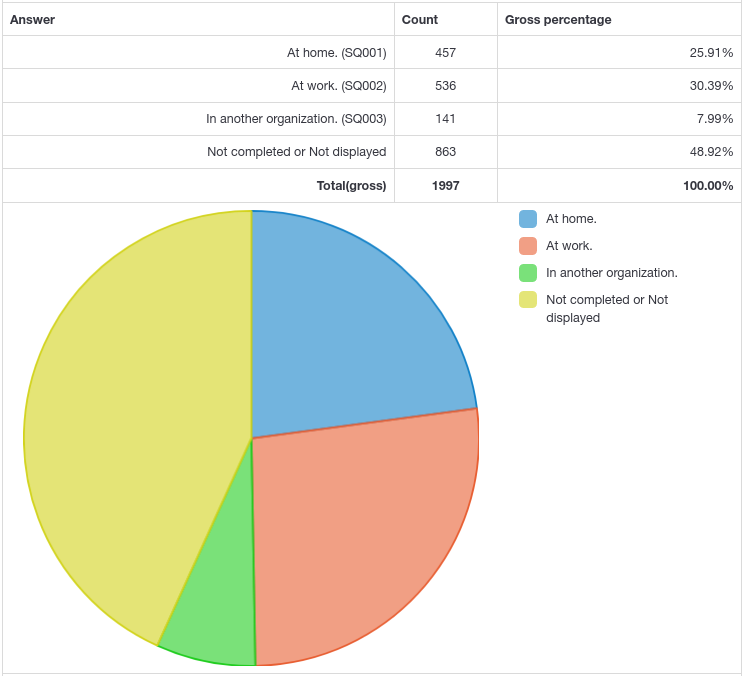
\includegraphics[width=16.5cm]{assets/8-summary.png}
\caption{Summary of Response 8}
\end{figure}

\newpage

\Large{\textbf{Question 9: If you use LTS at work or in an organization, how big is that organization?}}

\vspace{3mm}
\begin{figure}[h!]
\centering
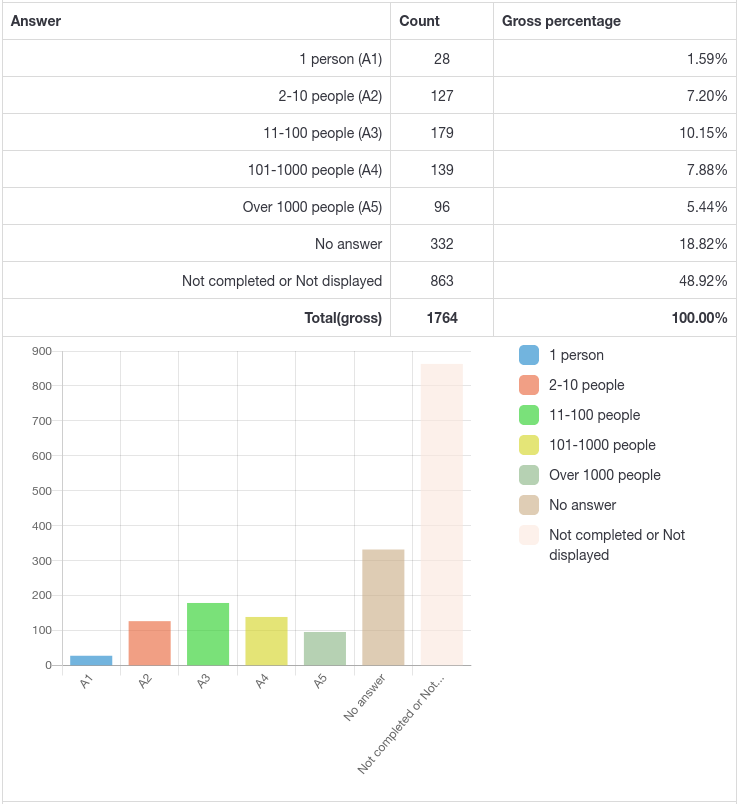
\includegraphics[width=16.5cm]{assets/9-summary.png}
\caption{Summary of Response 9}
\end{figure}

\newpage

\large{\textbf{Question 10: On a scale from 1 (= very unhappy) to 10 (= very happy), if your Debian duties
led you to interact with LTS contributors, how would you rate the interaction with said contributors?}}

\vspace{3mm}
\begin{figure}[h!]
\centering
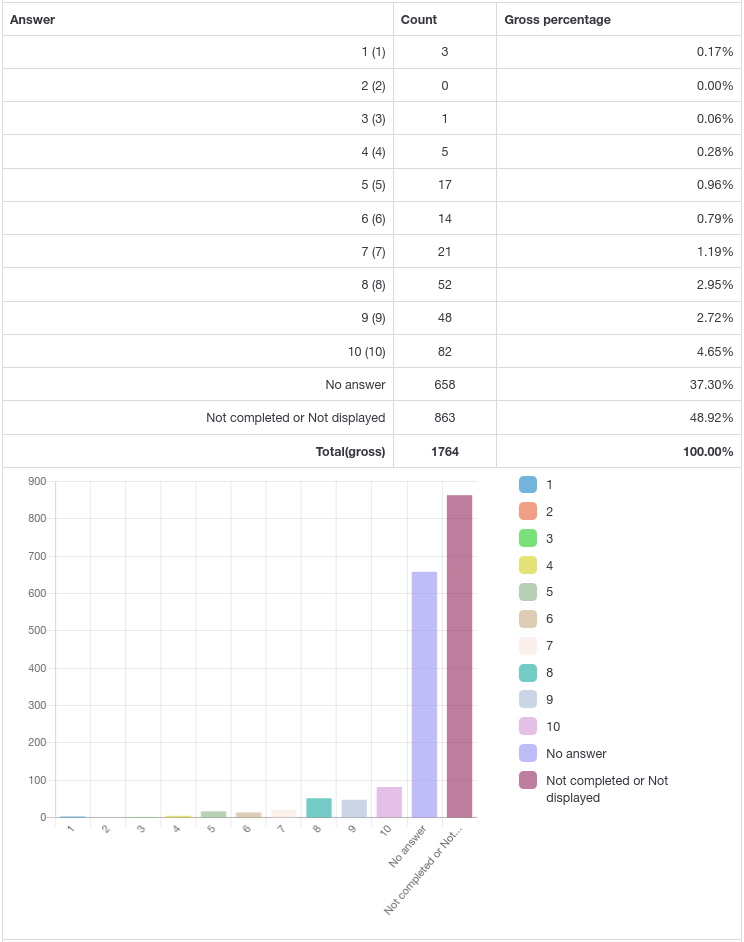
\includegraphics[width=16.3cm]{assets/10-summary.png}
\caption{Summary of Response 10}
\end{figure}

\newpage

\Large{\textbf{Question 11: How likely is it that you would recommend Debian LTS to a friend or
colleague? (1 = very unlikely, 10 = very likely)}}

\vspace{3mm}
\begin{figure}[h!]
\centering
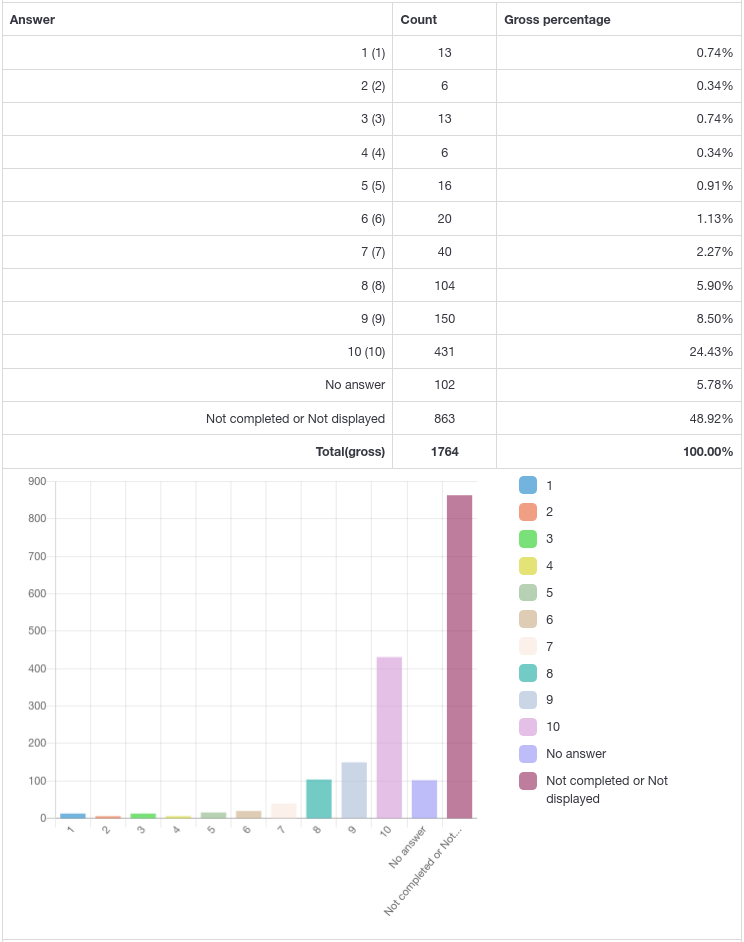
\includegraphics[width=16.3cm]{assets/11-summary.png}
\caption{Summary of Response 11}
\end{figure}

\end{document}
